\documentclass{article}
\usepackage{amsmath}
\usepackage{tikz}
\usetikzlibrary{arrows.meta}

\begin{document}

\begin{figure}[h]
    \centering
    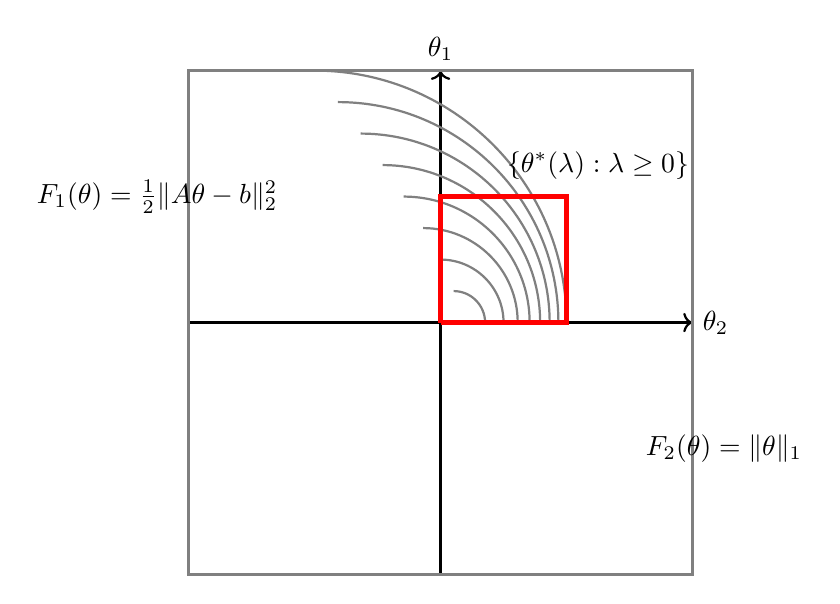
\begin{tikzpicture}[scale=0.8]
        % Axes
        \draw[->, thick] (-4,0) -- (4,0) node[right] {$\theta_2$};
        \draw[->, thick] (0,-4) -- (0,4) node[above] {$\theta_1$};

        % Contour lines for F1(theta)
        \foreach \i in {0.5, 1, 1.5, 2, 2.5, 3, 3.5, 4}
            \draw[thick, gray] ({sqrt(\i)},0) arc (0:90:\i);
        
        % Non-smooth objective function F2(theta)
        \draw[thick, gray] (-4,-4) -- (-4,4) -- (4,4) -- (4,-4) -- cycle;
        
        % Regularization path theta^*(lambda)
        \draw[red, ultra thick] (0,0) -- (0,2) -- (2,2) -- (2,0) -- (0,0);
        
        % Labels
        \node at (-4.5, 2) {$F_1(\theta) = \frac{1}{2}\|A\theta - b\|^2_2$};
        \node at (4.5, -2) {$F_2(\theta) = \|\theta\|_1$};
        \node at (2.5, 2.5) {$\{\theta^*(\lambda) : \lambda \geq 0\}$};
    \end{tikzpicture}
    \caption{Contour plot of smooth objective functions $F_1(\theta) = \frac{1}{2}\|A\theta - b\|^2_2$ and non-smooth objective function $F_2(\theta) = \|\theta\|_1$ in black and the \emph{regularization path} $\theta^*(\lambda) \in \text{argmin}_{\theta \in \mathbb{R}^n} \frac{1}{2}\|A\theta - b\|^2_2 + \lambda\|\theta\|_1$ in red.}
\end{figure}

\end{document}